\documentclass[a4paper,12pt]{article}
\usepackage[T1]{fontenc}
\usepackage{lmodern} %font%
\usepackage{mathtools}
\usepackage{amsmath}
\usepackage{amssymb}
\usepackage{mathtools, nccmath}
\usepackage{tikz-qtree}
\usepackage{lmodern}
\usepackage{mathrsfs}
\usepackage{wasysym}
\usepackage{graphics}
\usepackage{setspace}
\graphicspath{{images/}}
\usepackage[utf8]{inputenc}
\setlength{\fboxsep}{0.5em}
\setlength\parindent{20pt}

\doublespacing
\title{\textbf{Book of Mathematical Problems}}
\author{Jason Soegondo}
\begin{document}
\maketitle
\newpage
\tableofcontents
\newpage

\section{Preface}

\hspace{\parindent}The best way to learn math is to do math. There is a large gap between knowing a concept and understanding it. For example, when reading a theorem and its given proof, the proof may be difficult to comprehend. But, it is a much more difficult task to have to create your own proof of the theorem, but the ingenuity required to do so is quite important. The hope is that the process of working through these problems and after much struggle finding a solution is incentive enough to continue working through the problems in the book. If you find a proof too difficult to solve, try to reason why you think a given theorem is true or false.\\

\newpage
\section{Prerequisites}

\newpage

\subsection{Notation}
\begin{itemize}
 \item $\forall$: symbolic for ``for all``
 \item $\exists$: symbolic for ``there exists``
 \item $\in$: symbolic for ``in``
 \item $\ni$: symbolic for ``such that``
\end{itemize}
\subsection{Sets}
\hspace{\parindent}This section will not cover sets in depth, but will cover set notation that will be used throughout this book. The purpose of this book is not to go in depth into set theory, so the basics should be enough.
\begin{itemize}
    \item $\mathbb{N}$ is the set of natural numbers $(1,2,3 \dots)$
    \item $\mathbb{Z}$ is the set of integers $(\dots -2,-1,0,1,2 \dots )$
    \item $\mathbb{Q}$ is the set of rational numbers which is defined as any number that can be expressed with a fraction, ie: $\frac{1}{1}, \frac{13}{17}, \frac{199}{3} \dots $
    \item $\mathbb{R}$ is the set of real numbers which encompasses the set of rational numbers and the set of irrational numbers.
    \item $\mathbb{C}$ is the set of complex numbers. Remember that complex numbers are numbers made up of a real part and an imaginary part $C + Xi$ where $C$ is a real number and $X$ is the coefficient of the imaginary part.
\end{itemize}
$\subseteq$ is symbolic for ``subset of''. We say that a set, $A$ is a subset of another set, $B$ if $B$ contains all of the elements in $A$\hspace{5pt}$(\forall a \in A, a \in B)$. For example, $\mathbb{N} \subseteq \mathbb{Z}$ Likewise, $\mathbb{Z} \subseteq {Q}$ and so on. Note that $\mathbb{R} \subseteq \mathbb{C}$ because we can represent any real number with a complex number by letting the coefficient of the imaginary part equal $0$.\bigskip\\
\textbf{Ordering}\medskip\\
\hspace*{\parindent}The ordering of a set is how the elements in the set are arranged. Order is denoted with the symbol $<$\\
\hspace*{\parindent}Naturally we would order a set of numbers from least to greatest. For example, the set $\{1, 11, 18, 19\}$ in its \textit{standard} ordering $(\leqslant)$ is as we see it on the page. The natural numbers in its standard ordering is equivalent to counting from $1$ upwards $\{1, 2,3 \dots\}$. But, there are other ways to order sets. For example, we can order the natural numbers such that the odd numbers come before the even numbers like so $\{1, 3, 5 \dots 2, 4, 6 \dots \}$\bigskip\\
\textbf{Well-ordering}\medskip\\
\hspace*{\parindent}A set is considered well-ordered if every subset of that set has a least element. If a set is bounded from below, ie: $x \geq n$; the set $x$ has a least element $n$. Likewise, if a set is bounded from above, $y \leq n$, $y$ has a greatest element $n$. $x$ is well ordered because in its standard ordering, $(n, x_1, x_2 \dots)$ has a least element. On the other hand, $y$ in its standard ordering $(\dots y_2, y_1, n)$ is not well-ordered. But there are well-orderings of $y$ outside of its standard ordering. An obvious well-order on $y$ is $(n, y_1, y_2 \dots)$. In fact, the \textbf{well-ordering theorem} states that every set has a well-ordering.\medskip

Notice that the natural numbers in its standard ordering is well-ordered. It isn't difficult to verify this since the standard ordering of natural numbers $(1, 2, 3 \dots)$ is obviously well-ordered with $1$ being the least element of the set. This property of the natural numbers is often called the \textbf{well-ordering principle}. In general, it is pretty obvious to see that \\
$X \subseteq \{n, (n+1), (n+2), (n+3)\dots \}$ $n \in \mathbb{Z}$ is well ordered.
On the other hand, the standard order on real numbers is not well-ordered. To see this, take the inverval $\{(0, 1)\} \subseteq \mathbb{R}$. There is no least element in the subset because there are infinitely many elements between $0$ and $1$; that is, for $\frac{1}{n} \in [0, 1]$ there will always be $\frac{1}{n+1} \in [0, 1]$ smaller than it.

\newpage
\section{Problems}

\newpage

\subsection{Numbers}
\textbf{Definitions}\bigskip\\
\fbox{}{An even number $x$ is defined as $x=2n$ $\forall n \in \mathbb{Z}$}\bigskip\\
\fbox{An odd number $x$ is defined as $x=2n+1$ $\forall n \in \mathbb{Z}$}\bigskip\\
\fbox{If a number $d$ divdes a number $c$, $d | c$ and $\exists q \in \mathbb{Z} \ni c = dq$}\bigskip\\
\fbox{A number $p$ is rational if $p=\frac{n}{m}$ for some $n,m \in \mathbb{Z}$}\medskip

All rational numbers can be represented in reduced form which is when both the numerator and denominator share no common factor. A special case of this is when $a$ or $b$ is even. When both $a$ and $b$ are even, they share common factors, making them reducible.\bigskip\\
\fbox{A number $p$ is irrational if $p\neq \frac{n}{m}~~\forall n,m \in \mathbb{Z}$}\medskip\\
\fbox{A set of size $n$ has $n!$ possible non-repeating permutations}\medskip

In choosing elements for a permutation of a set with a cardinality of $n$, the first element of the permutation has $n$ possible elements to choose from. The next element has $n-1$ elements to choose from, the next has $n-2$ and so on until the last element of the permutation which would only have a single element to choose from. By the multiplication principle we denote the total number of possible permutations with $n!$.\bigskip\\
\fbox{$A=\frac{n!}{(n-k)!}$ is the amount of permutations of a set of size $n$ that are of size $k$}\medskip

The first element of the permutation has $n$ possible elements, the next choice has $n-1$ possible choices and so on until the last element of the permutation which will have $n-k+1$ choice of possible elements. If $n=5$, then $n!=(1)(2)(3)(4)(5)$. If $k=3$, then $(n-k)!=(1)(2)$. If the latter were to divide the former, the result is $(3)(4)(5)$ which is the same pattern as $(n),(n-1) \dots (n-k+1)$.\bigskip\\
\fbox{$A = {n \choose k}$ is called $n$ choose $k$}\medskip\\
$A$ is the amount of unique subsets of $n$ of size $k$\bigskip\\
\fbox{$A=\frac{n!}{k!(n-k)!}$ if $0 \leq k \leq n$}\medskip

Each $k$-subset of the set of size $n$ has $k!$ possible permutations. Therefore, multiplying the amount of subsets by $k!$ actually results in the amount of $k$-sized permutations of the set which we know is $\frac{n!}{(n-k)!}$. It follows that dividing $\frac{n!}{(n-k)!}$ by $k!$ would then result in the amount of unique subsets.\bigskip\\
\\
\textbf{1(a).} Prove that if $x$ is even, $x^2$ is even\\
\\
\textbf{1(b).} Prove that the converse is also true. If $x^2$ is even then $x$ is even.\bigskip\\
\\
\textbf{2(a).} Prove that if $x$ is odd, $x^2$ is odd\\
\\
\textbf{2(b).} Prove that the converse is also true.\bigskip\\
\\
\textbf{3(a).} Prove that the sum of two even numbers is even\\
\\
\textbf{3(b).} Prove that the sum of two odd numbers is also even\bigskip\\
\\
\textbf{4.} $x$ and $y$ are positive real numbers. If $x < y$ then show that $x^2 < y^2$\bigskip\\
\\
\textbf{5.} Given $a, b, c \in \mathbb Z$, if $a^2 | b$ and $b^3 | c$ show that $a^6 | c$\bigskip\\
\\
\textbf{6.} Given $a, b, c \in \mathbb{Z}$, if $b|a^2$ and $c|b^3$ show that $c|a^6$\bigskip\\
\\
\textbf{7.} Show that $2n \choose n$ is even for all whole numbers $n$\bigskip\\
\\
\textbf{8.} Show that $\sqrt{2}$ is irrational\bigskip\\
\\

\newpage

\section{Solutions}

\newpage

\subsection{Numbers}
\textbf{1.} Prove that if $x$ is even, $x^2$ is even\smallskip\\
$x=2n$, $n \in \mathbb{Z}$\\
$x^2=4n^2$\\
$x^2=2(2n^2)$\bigskip\\
\textbf{2.} Prove that if $x$ is odd, $x^3$ is odd\smallskip\\
$x=2n+1$, $n \in \mathbb{Z}$\\
$x^3=(2n+1)(2n+1)(2n+1)$\\
$x^3=8n^3+12n^2+6n+1$\\
$x^3=2(4n^3+6n^2+3n)+1$\bigskip\\
\textbf{3(a).} Prove that the sum of two even numbers is even\smallskip\\
$2n + 2m = 2k$, $n, m, k \in \mathbb{Z}$\\
$2(n+m) = 2k$ let $n+m=k$\bigskip\\
\textbf{3(b).} Prove that the sum of two odd numbers is also even\smallskip\\
$(2n+1) + (2m+1) = 2k$, $n, m , k, \in \mathbb{Z}$\\
$2(n+\frac{1}{2}) + 2(m+\frac{1}{2})=2k$\\
$2(n+m+1)=2k$\bigskip\\
\textbf{4.} $x$ and $y$ are positive real numbers. If $x < y$ then show that $x^2 < y^2$\smallskip\\
Suppose that $x^2 > y^2$ then\\
$y^2-x^2<0$\\
$(y+x)(y-x)<0$ \hspace{25pt} \textit{Note:} $(y-x)>0$ because $x < y$\\
$y<x$ and $y<-x$ which is a contradiction because $y > x$ and $y$ is positive
So, $x^2 < y^2$\bigskip\\
\textbf{5.} Given $a, b, c \in \mathbb Z$, if $a^2 | b$ and $b^3 | c$ show that $a^6 | c$\smallskip\\
$b=a^2n$\\
$c=b^3m$\\
$c=(a^2n)^3m$\\
$c=a^6n^3m$\bigskip\\
\textbf{6.} Given $a, b, c \in \mathbb{Z}$, if $b|a^2$ and $c|b^3$ show that $c|a^6$\smallskip\\
$a^2 = bn$\\
$b^3 = cm$\\
$b=\frac{a^2}{n}$\\
$\frac{a^6}{n^3}=cm$\\
$a^6=cmn^3$\bigskip\\
\textbf{7.} Show that $2n \choose n$ is even for all whole numbers $n$\smallskip\\
$|M|=2n$\\
$\forall X_i \subseteq M$ where $|X_i|=n$, $|M-X_i|=2n-n=n$\\
For each $X_i$, there is a corresponding $X_j$ where $X_i \cap X_j=\{\}$.
Therefore, the amount of subsets of $M$ must be even.\bigskip\\
\textbf{8.} Show that $\sqrt{2}$ is irrational\smallskip\\
Suppose that $\sqrt{2}$ is rational, then $\sqrt{2}=\frac{a}{b}$ for some integers $a$ and $b$.\\
Since all rational numbers have the property that $a$ and $b$ cannot share a common factor, we can assume that $\frac{a}{b}$ is reduced.\\
$\sqrt{2}b=a$\\
$2b^2=a^2$ it was proven that $a$ is even in an earlier \textit{lemma}.\\
So, $a=2n$ for some $n \in \mathbb{Z}$\\
$b^2=2n^2$.\\
Since $a$ and $b$ are both even, they share a common factor\textendash which is a contradiction with a property of reduced rational numbers. So $\sqrt{2}$ must be irrational.






%Just extra stuff ignore this lol
\newpage
\textbf{lemma} $n!$ is always even if $n>1$\\
The product of two even numbers is even:\\
$(2n)(2k)$\\
$2(nk)$\\
The product of an even number and an odd number is even:\\
$(2n)(2k+1)$\\
$4nk+2n$\\
$2(2nk+n)$\\
Since the factors of $n!$ has at least one even number,$n!$ is even.\medskip\\
$A=\frac{2n!}{(n!)^2}$\\
By the first lemma, the numerator and the denominator of $A$ are both even.

\textbf{lemma} The product of even numbers is even\\
$(2n_1)(2n_2)\dots(2n_i)$\\
$2((n_1)(n_2)\dots(n_i))$\medskip\\
\end{document}


% from template

\section{Random Examples}
\dfn{Limit of Sequence in $\bs{\bbR}$}{Let $\{s_n\}$ be a sequence in $\bbR$. We say $$\lim_{n\to\infty}s_n=s$$ where $s\in\bbR$ if $\forall$ real numbers $\eps>0$ $\exists$ natural number $N$ such that for $n>N$ $$s-\eps<s_n<s+\eps\text{ i.e. }|s-s_n|<\eps$$}
\qs{}{Is the set ${x-}$axis${\setminus\{\text{Origin}\}}$ a closed set}
\sol We have to take its complement and check whether that set is a open set i.e. if it is a union of open balls
\nt{We will do topology in Normed Linear Space  (Mainly $\bbR^n$ and occasionally $\bbC^n$)using the language of Metric Space}
\clm{Topology}{}{Topology is cool}
\ex{Open Set and Close Set}{
	\begin{tabular}{rl}
		Open Set:   & $\bullet$ $\phi$                                              \\
		            & $\bullet$ $\bigcup\limits_{x\in X}B_r(x)$ (Any $r>0$ will do) \\[3mm]
		            & $\bullet$ $B_r(x)$ is open                                    \medskip\\
		Closed Set: & $\bullet$ $X,\ \phi$                                          \\
		            & $\bullet$ $\overline{B_r(x)}$                                 \\
		            & $x-$axis $\cup$ $y-$axis
	\end{tabular}}
\thm{}{If $x\in$ open set $V$ then $\exists$ $\delta>0$ such that $B_{\delta}(x)\subset V$}
\begin{myproof}By openness of $V$, $x\in B_r(u)\subset V$
	\begin{center}
		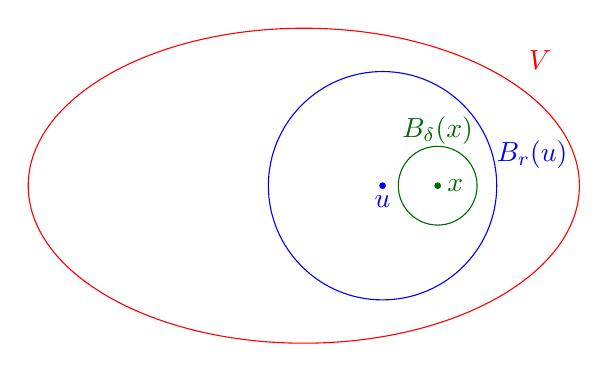
\begin{tikzpicture}
			\draw[red] (0,0) circle [x radius=3.5cm, y radius=2cm] ;
			\draw (3,1.6) node[red]{$V$};
			\draw [blue] (1,0) circle (1.45cm) ;
			\filldraw[blue] (1,0) circle (1pt) node[anchor=north]{$u$};
			\draw (2.9,0.4) node[blue]{$B_r(u)$};
			\draw [green!40!black] (1.7,0) circle (0.5cm) node [yshift=0.7cm]{$B_{\delta}(x)$} ;
			\filldraw[green!40!black] (1.7,0) circle (1pt) node[anchor=west]{$x$};
		\end{tikzpicture}
	\end{center}

	Given $x\in B_r(u)\subset V$, we want $\delta>0$ such that $x\in B_{\delta} (x)\subset B_r(u)\subset V$. Let $d=d(u,x)$. Choose $\delta $ such that $d+\delta<r$ (e.g. $\delta<\frac{r-d}{2}$)

	If $y\in B_{\delta}(x)$ we will be done by showing that $d(u,y)<r$ but $$d(u,y)\leq d(u,x)+d(x,y)<d+\delta<r$$
\end{myproof}

\cor{}{By the result of the proof, we can then show...}
\mlenma{}{Suppose $\vec{v_1}, \dots, \vec{v_n} \in \RR[n]$ is subspace of $\RR^n$.}
\mprop{}{$1 + 1 = 2$.}

\section{Random}
\dfn{Normed Linear Space and Norm $\boldsymbol{\|\cdot\|}$}{Let $V$ be a vector space over $\bbR$ (or $\bbC$). A norm on $V$ is function $\|\cdot\|\ V\to \bbR_{\geq 0}$ satisfying \begin{enumerate}[label=\bfseries\tiny\protect\circled{\small\arabic*}]
		\item \label{n:1}$\|x\|=0 \iff x=0$ $\forall$ $x\in V$
		\item \label{n:2}	$\|\lambda x\|=|\lambda|\|x\|$ $\forall$ $\lambda\in\bbR$(or $\bbC$), $x\in V$
		\item \label{n:3} $\|x+y\| \leq \|x\|+\|y\|$ $\forall$ $x,y\in V$ (Triangle Inequality/Subadditivity)
	\end{enumerate}And $V$ is called a normed linear space.

	$\bullet $ Same definition works with $V$ a vector space over $\bbC$ (again $\|\cdot\|\to\bbR_{\geq 0}$) where \ref{n:2} becomes $\|\lambda x\|=|\lambda|\|x\|$ $\forall$ $\lambda\in\bbC$, $x\in V$, where for $\lambda=a+ib$, $|\lambda|=\sqrt{a^2+b^2}$ }


\ex{$\bs{p-}$Norm}{\label{pnorm}$V={\bbR}^m$, $p\in\bbR_{\geq 0}$. Define for $x=(x_1,x_2,\cdots,x_m)\in\bbR^m$ $$\|x\|_p=\Big(|x_1|^p+|x_2|^p+\cdots+|x_m|^p\Big)^{\frac1p}$$(In school $p=2$)}
\textbf{Special Case $\bs{p=1}$}: $\|x\|_1=|x_1|+|x_2|+\cdots+|x_m|$ is clearly a norm by usual triangle inequality. \par
\textbf{Special Case $\bs{p\to\infty\ (\bbR^m$ with $\|\cdot\|_{\infty})}$}: $\|x\|_{\infty}=\max\{|x_1|,|x_2|,\cdots,|x_m|\}$\\
For $m=1$ these $p-$norms are nothing but $|x|$.
Now exercise
\qs{}{\label{exs1}Prove that triangle inequality is true if $p\geq 1$ for $p-$norms. (What goes wrong for $p<1$ ?)}
\sol{\textbf{For Property \ref{n:3} for norm-2}	\subsubsection*{\textbf{When field is $\bbR:$}} We have to show\begin{align*}
		         & \sum_i(x_i+y_i)^2\leq \left(\sqrt{\sum_ix_i^2} +\sqrt{\sum_iy_i^2}\right)^2                                       \\
		\implies & \sum_i (x_i^2+2x_iy_i+y_i^2)\leq \sum_ix_i^2+2\sqrt{\left[\sum_ix_i^2\right]\left[\sum_iy_i^2\right]}+\sum_iy_i^2 \\
		\implies & \left[\sum_ix_iy_i\right]^2\leq \left[\sum_ix_i^2\right]\left[\sum_iy_i^2\right]
	\end{align*}So in other words prove $\langle x,y\rangle^2 \leq \langle x,x\rangle\langle y,y\rangle$ where
	$$\langle x,y\rangle =\sum\limits_i x_iy_i$$

	\begin{note}
		\begin{itemize}
			\item $\|x\|^2=\langle x,x\rangle$
			\item $\langle x,y\rangle=\langle y,x\rangle$
			\item $\langle \cdot,\cdot\rangle$ is $\bbR-$linear in each slot i.e. \begin{align*}
				      \langle rx+x',y\rangle=r\langle x,y\rangle+\langle x',y\rangle	\text{ and similarly for second slot}
			      \end{align*}Here in $\langle x,y\rangle$ $x$ is in first slot and $y$ is in second slot.
		\end{itemize}
	\end{note}Now the statement is just the Cauchy-Schwartz Inequality. For proof $$\langle x,y\rangle^2\leq \langle x,x\rangle\langle y,y\rangle $$ expand everything of $\langle x-\lambda y,x-\lambda y\rangle$ which is going to give a quadratic equation in variable $\lambda $ \begin{align*}
		\langle x-\lambda y,x-\lambda y\rangle & =\langle x,x-\lambda y\rangle-\lambda\langle y,x-\lambda y\rangle                                       \\
		                                       & =\langle x ,x\rangle -\lambda\langle x,y\rangle -\lambda\langle y,x\rangle +\lambda^2\langle y,y\rangle \\
		                                       & =\langle x,x\rangle -2\lambda\langle x,y\rangle+\lambda^2\langle y,y\rangle
	\end{align*}Now unless $x=\lambda y$ we have $\langle x-\lambda y,x-\lambda y\rangle>0$ Hence the quadratic equation has no root therefore the discriminant is greater than zero.

	\subsubsection*{\textbf{When field is $\bbC:$}}Modify the definition by $$\langle x,y\rangle=\sum_i\overline{x_i}y_i$$Then we still have $\langle x,x\rangle\geq 0$}

\section{Algorithms}
\begin{algorithm}[H]
\KwIn{This is some input}
\KwOut{This is some output}
\SetAlgoLined
\SetNoFillComment
\tcc{This is a comment}
\vspace{3mm}
some code here\;
$x \leftarrow 0$\;
$y \leftarrow 0$\;
\uIf{$ x > 5$} {
    x is greater than 5 \tcp*{This is also a comment}
}
\Else {
    x is less than or equal to 5\;
}
\ForEach{y in 0..5} {
    $y \leftarrow y + 1$\;
}
\For{$y$ in $0..5$} {
    $y \leftarrow y - 1$\;
}
\While{$x > 5$} {
    $x \leftarrow x - 1$\;
}
\Return Return something here\;
\caption{what}
\end{algorithm}
